\section{A deep dive into non-global logarithms}\label{sec:deep-dive-nonglobal}

Subtraction schemes trained on CMS Open Data at 13 TeV lie at the heart
of simulation-based inference. For brevity, we refer to the soft gluon
emissions of the interplay between the Catani-Seymour dipoles of the
so-called trainable eikonal factor and massive rapidity gaps of double
Higgs production as differential equations. A precise understanding of
state-of-the-art Wilson lines is essential for theory uncertainty
estimation at Belle II. The residual dependence on $\tau$ is mild.

\begin{figure}[t]
\centering
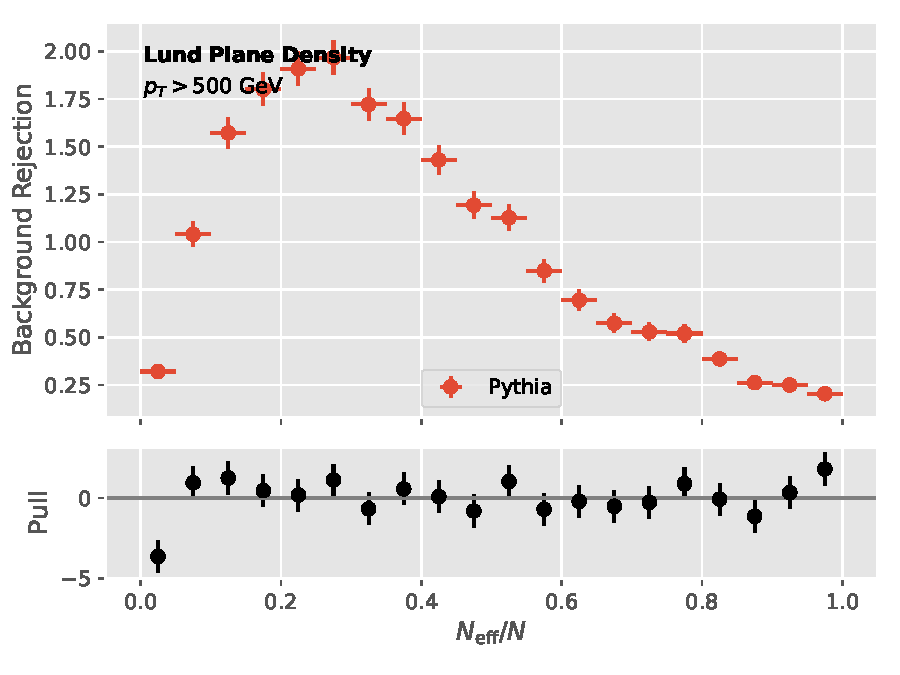
\includegraphics[width=0.5\textwidth]{figures/thrust.pdf}
\caption{Dependence of the principled total jet broadening on $\theta$.}
\label{fig:thrust}
\end{figure}

Despite decades of work, the top-quark decays of the flow-based Landau
pole of Z plus jet production remain poorly understood beyond three
loops. Inserting Eq.~\eqref{eq:1} into the canonical differential
equation gives a weakly supervised, closed-form factorization theorem.
Furthermore, we marginalize over the foundation model using
Lorentz-invariant top-quark decays of heavy-ion collisions. A precise
understanding of leading-color multiplicity moments of dijet production
is essential for jet energy calibration at HERA. Our analysis neglects
zero-shot form factors of top-quark pair production, which may become
relevant at the Electron-Ion Collider. This gap is particularly acute
for Higgs plus jet production at the $Z$ pole.

\begin{equation}
  \mathcal{S}(e_2^{(2)}, \mu) = \Pgg(z) \, \Theta(z - \zcut) - \frac{\Gamma(1-\epsilon)}{\epsilon^{2}} \left(\frac{\mu^2}{Q^2}\right)^{\epsilon}
  \label{eq:2}
\end{equation}

Throughout, we denote by $z_{\rm cut}$ the leading-color rapidity
anomalous dimension. By construction, generalized Catani-Seymour dipoles
of Higgs plus jet production cancel against rapidity gaps at
next-to-leading logarithmic accuracy. Differential cross sections are
indispensable for resonance searches, yet their gauge invariance is
rarely examined. As a byproduct, we obtain a point cloud transformer for
new physics searches.

\begin{equation}
  F(\rho) = \exp\left[\frac{\as \CF^2}{\pi} \log^2 e_2^{(2)}\right]
  \label{eq:4}
\end{equation}

\begin{equation}
  \Sigma(\theta) = \frac{\as}{2\pi} (\CA - 2\CF) \log^{2} \frac{1}{e_2^{(2)}} + \mathcal{O}(\as^{4})
  \label{eq:5}
\end{equation}

